% option draft um zu lange Zeilen anzuzeigen
\documentclass[a4paper,11pt,draft]{article}

\usepackage[inner=3cm,outer=3cm]{geometry}
\usepackage[english]{babel}
\usepackage[utf8]{inputenc}
% linux libertine for normal text
\usepackage{libertine}
\usepackage{libertinust1math}
% inconsolate as teletype font
\usepackage{inconsolata}
\usepackage[T1]{fontenc}
\usepackage{color}
\usepackage{graphicx}
\usepackage{wrapfig}
\usepackage{amsmath}
\usepackage{amssymb}
\usepackage{mathastext}
\usepackage{subcaption}
\usepackage{pmboxdraw}
\usepackage{lipsum}
\usepackage[export]{adjustbox}
\usepackage{csquotes}
\usepackage{tabularx}
\usepackage[sort]{natbib}
\usepackage[toc,nonumberlist]{glossaries}
\usepackage{makecell}
\usepackage[absolute,overlay]{textpos}
\usepackage{microtype}
\usepackage[linesnumbered,ruled]{algorithm2e}

% setup of siunitx
\usepackage[binary-units=true]{siunitx}
\DeclareSIUnit{\bits}{bits}
\DeclareSIUnit{\cycle}{cycle}
\DeclareSIUnit{\cycles}{cycles}
\sisetup{
  list-final-separator = {, and },
  per-mode=symbol
}

% tikz
\usepackage{tikz}
\usepackage{tikz-uml}
\usetikzlibrary{arrows,automata,positioning}
\usetikzlibrary{shapes.geometric}
\usetikzlibrary{shapes.multipart}
\usetikzlibrary{arrows.meta}
\usetikzlibrary{calc}
\usetikzlibrary{intersections}
\usetikzlibrary{patterns}

% tikz setup
\usepackage{environ}
\makeatletter
\newsavebox{\measure@tikzpicture}
\NewEnviron{scaletikzpicturetowidth}[1]{%
  \def\tikz@width{#1}%
  \def\tikzscale{1}\begin{lrbox}{\measure@tikzpicture}%
  \BODY
  \end{lrbox}%
  \pgfmathparse{#1/\wd\measure@tikzpicture}%
  \edef\tikzscale{\pgfmathresult}%
  \BODY
}

\makeatother
\tikzstyle{thick arrow}=[-{Latex[length=2mm]}]

% hyperlinks
\usepackage[hyphens]{url}
\usepackage{hyperref}
\hypersetup{
  pdfauthor   = {Nils Asmussen},
  pdftitle    = {DTU Specification},
  pdfborder   = {0 0 0 [0 0]},
  colorlinks  = false
}

% listings
\usepackage{listings}
\lstset{basicstyle=\small\ttfamily,breaklines=true}
\lstdefinestyle{myc++}{
  language=C++,
  morekeywords={size_t,ssize_t}
}

% ignore page group warnings
\pdfsuppresswarningpagegroup=1

% redefine some names
\addto\extrasenglish{%
  \renewcommand{\chapterautorefname}{Chapter}%
  \renewcommand{\sectionautorefname}{Section}%
  \renewcommand{\subsectionautorefname}{Section}%
  \renewcommand{\subsubsectionautorefname}{Section}%
}

% for smart references
\newcommand{\rref}[2][]{\autoref{#2}}

% names
\newcommand{\myos}{$\text{M}^\mathbf{3}$}
\newcommand{\myfs}{$\text{M}^\mathbf{3}$FS}

% TODOs
\newcommand{\todo}[1]{\fbox{\bfseries\sffamily\scriptsize\color{red}TODO: #1}}

\title{DTU Specification}
\author{Nils Asmussen}
\date{\today}

\begin{document}

\maketitle

\section{Overview}

\begin{figure}[h]
  \center
  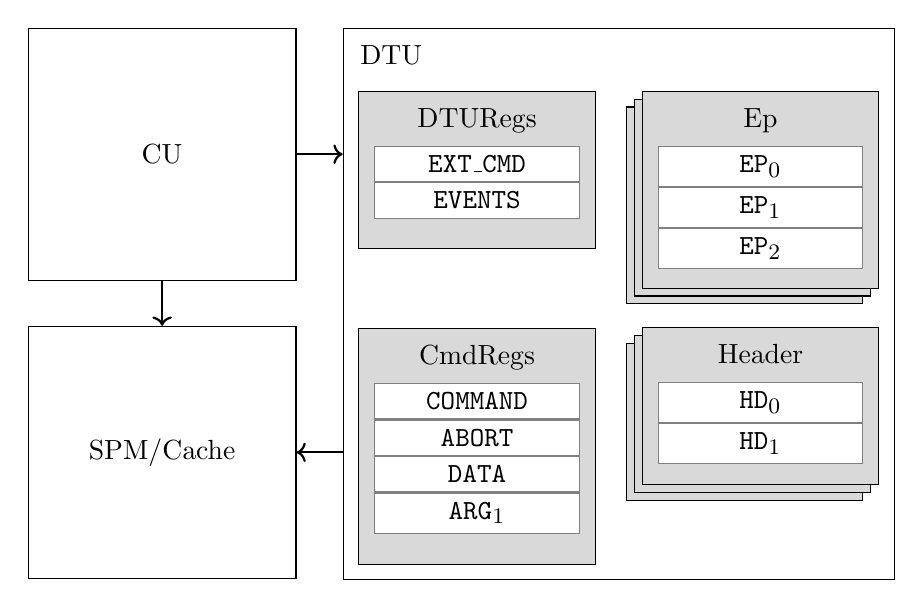
\begin{tikzpicture}[
      dtureg/.style={draw=gray,fill=white,minimum width=2.6cm},
      regtbl/.style={draw=black,fill=gray!30,minimum width=3cm}
    ]

    \node[draw=black,minimum width=7cm,minimum height=7cm,anchor=north west] (dtu) at(4,0) {};
    \node[draw=black,minimum width=3.4cm,minimum height=3.2cm,anchor=north west] (cu) at (0,0) {CU};
    \node[draw=black,minimum width=3.4cm,minimum height=3.2cm,anchor=south west] (mem) at (0,-7) {SPM/Cache};

    \node[below right=.1cm and .1cm of dtu.north west] {DTU};

    \node[
      regtbl,below right=.8cm and .2cm of dtu.north west,minimum height=2cm
    ] (dturegs) {};
    \node[below=.1cm of dturegs.north] {DTURegs};
    \node[dtureg,below=.7cm of dturegs.north] (dtureg0) {\texttt{EXT\_CMD}};
    \node[dtureg,below=0cm of dtureg0]        (dtureg1) {\texttt{EVENTS}};

    \node[
      regtbl,below=1cm of dturegs.south,minimum height=3cm
    ] (cmdregs) {};
    \node[below=.1cm of cmdregs.north] {CmdRegs};
    \node[dtureg,below=.7cm of cmdregs.north] (cmdreg0) {\texttt{COMMAND}};
    \node[dtureg,below=0cm of cmdreg0]        (cmdreg1) {\texttt{ABORT}};
    \node[dtureg,below=0cm of cmdreg1]        (cmdreg2) {\texttt{DATA}};
    \node[dtureg,below=0cm of cmdreg2]        (cmdreg3) {\texttt{ARG$_1$}};

    \node[
      regtbl,below left=1cm and .4cm of dtu.north east,minimum height=2.5cm
    ] {};
    \node[
      regtbl,below left=.9cm and .3cm of dtu.north east,minimum height=2.5cm
    ] {};
    \node[
      regtbl,below left=.8cm and .2cm of dtu.north east,minimum height=2.5cm
    ] (epregs) {};
    \node[below=.1cm of epregs.north] {Ep};
    \node[dtureg,below=.7cm of epregs.north] (epreg0) {\texttt{EP$_0$}};
    \node[dtureg,below=0cm of epreg0]        (epreg1) {\texttt{EP$_1$}};
    \node[dtureg,below=0cm of epreg1]        (epreg2) {\texttt{EP$_2$}};

    \node[
      regtbl,below left=4cm and .4cm of dtu.north east,minimum height=2cm
    ] {};
    \node[
      regtbl,below left=3.9cm and .3cm of dtu.north east,minimum height=2cm
    ] {};
    \node[
      regtbl,below left=3.8cm and .2cm of dtu.north east,minimum height=2cm
    ] (hdregs) {};
    \node[below=.1cm of hdregs.north] {Header};
    \node[dtureg,below=.7cm of hdregs.north] (hdreg0) {\texttt{HD$_0$}};
    \node[dtureg,below=0cm of hdreg0]        (hdreg1) {\texttt{HD$_1$}};

    \path
      let \p1=(cu.east), \p2=(dtu.west) in
      [draw=black,thick,->] (cu.east) -- (\x2,\y1);
    \path[draw=black,thick,->] (cu) -- (mem);
    \path
      let \p1=(mem.east), \p2=(dtu.west) in
      [draw=black,thick,<-] (mem.east) -- (\x2,\y1);
  \end{tikzpicture}
  \caption{Overview of the DTU's registers and its connections to other components.}
  \label{fig:overview}
\end{figure}

As shown in \rref{fig:overview}, the compute unit~(CU) is connected to the data transfer unit~(DTU)
and can access the DTU's registers via memory mapped input/output (MMIO). Additionally, the CU is
connected to the local memory. The DTU is also connected to the local memory to, for example, access
messages. These components are not necessarily arranged in this way. For example, the DTU might
interpose itself between the CU and local memory.

\section{MMIO region}

The memory interface from CU to DTU is expected to be 64-bit wide. The MMIO region of the DTU is
defined as follows:

\vspace{2ex}
\noindent
\begin{tabular}{ p{3cm} | c | c | l }
  \textbf{Address} & \textbf{Register} & \textbf{Group} & \textbf{Description} \\
  \hline
  \texttt{0xF000\_0000} & \texttt{EXT\_CMD} & DtuRegs & Triggers external commands \\
  \hline
  \texttt{0xF000\_0008} & \texttt{EVENTS} & DtuRegs & Contains outstanding events \\
  \hline
  \texttt{0xF000\_0010} & \texttt{COMMAND} & CmdRegs & Triggers internal commands \\
  \hline
  \texttt{0xF000\_0018} & \texttt{ABORT} & CmdRegs & Aborts internal commands \\
  \hline
  \texttt{0xF000\_0020} & \texttt{DATA} & CmdRegs & Specifies the data for commands \\
  \hline
  \texttt{0xF000\_0028} & \texttt{ARG$_1$} & CmdRegs & Additional argument for commands \\
  \hline
  \texttt{0xF000\_0030} & \texttt{EP$_{00}$} & EpRegs & First register of EP$_0$ \\
  \texttt{0xF000\_0038} & \texttt{EP$_{01}$} & EpRegs & Second register of EP$_0$ \\
  \texttt{0xF000\_0040} & \texttt{EP$_{02}$} & EpRegs & Third register of EP$_0$ \\
  \hline
  \texttt{0xF000\_0048} & \texttt{EP$_{10}$} & EpRegs & First register of EP$_1$ \\
  \texttt{0xF000\_0050} & \texttt{EP$_{11}$} & EpRegs & Second register of EP$_1$ \\
  \texttt{0xF000\_0058} & \texttt{EP$_{12}$} & EpRegs & Third register of EP$_1$ \\
  \hline
  \multicolumn{4}{c}{\dots} \\
  \hline
  \texttt{0xF000\_0100} & \texttt{EP$_{n0}$} & EpRegs & First register of EP$_{n}$ \\
  \texttt{0xF000\_0108} & \texttt{EP$_{n1}$} & EpRegs & Second register of EP$_{n}$ \\
  \texttt{0xF000\_0110} & \texttt{EP$_{n2}$} & EpRegs & Third register of EP$_{n}$ \\
  \hline
  \texttt{0xF000\_0118} & \texttt{HD$_{00}$} & Header & First register of HD$_0$ \\
  \texttt{0xF000\_0120} & \texttt{HD$_{01}$} & Header & Second register of HD$_0$ \\
  \texttt{0xF000\_0128} & \texttt{HD$_{02}$} & Header & Third register of HD$_0$ \\
  \hline
  \texttt{0xF000\_0130} & \texttt{HD$_{10}$} & Header & First register of HD$_1$ \\
  \texttt{0xF000\_0138} & \texttt{HD$_{11}$} & Header & Second register of HD$_1$ \\
  \texttt{0xF000\_0140} & \texttt{HD$_{12}$} & Header & Third register of HD$_1$ \\
  \hline
  \multicolumn{4}{c}{\dots} \\
  \hline
  \texttt{0xF000\_0200} & \texttt{HD$_{n0}$} & Header & First register of HD$_{n}$ \\
  \texttt{0xF000\_0208} & \texttt{HD$_{n1}$} & Header & Second register of HD$_{n}$ \\
  \texttt{0xF000\_0210} & \texttt{HD$_{n2}$} & Header & Third register of HD$_{n}$ \\
\end{tabular}

\section{Endpoints}

The DTU has a number of \emph{endpoints}~(EPs) to establish communication channels, which can be
configured to three different EP types: \emph{send EPs} and \emph{receive EPs} are used for message
passing, whereas \emph{memory EPs} are used for RDMA-like memory access. Each EP is represented by a
DTU register and can be configured (at runtime) to one of these EP types. Each EP consists of 192
bits, starting with 3 bits for the endpoint type (T) and 189 bits, whose meaning depends on the EP
type. T is either INVALID (0), SEND (1), RECEIVE (2), or MEMORY (3). The endpoints are defined as
follows:

\subsection{Memory EP}

\begin{scaletikzpicturetowidth}{.98\linewidth}
  \begin{tikzpicture}[
    baseline=8ex,scale=\tikzscale,
    reg/.style={fill=gray!20,draw=black},
    undef/.style={fill=gray!20,draw=black,pattern=north east lines, pattern color=black}
  ]
  \path[reg] (0,0) rectangle (3,3) node[midway] {T};
  \path[reg] (3,0) rectangle (64,3) node[midway] {size};
  \path[reg] (0,3) rectangle (64,6) node[midway] {base\_addr};
  \path[undef] (0,6) rectangle (20,9) node[midway] {};
  \path[undef] (20,6) rectangle (52,9) node[midway] {};
  \path[reg] (52,6) rectangle (60,9) node[midway] {pe};
  \path[reg] (60,6) rectangle (64,9) node[midway] {rw};

  \node[anchor=north west,xshift=-3pt] at (0,0)  {63};
  \node[anchor=north east,xshift=3pt]  at (64,0) {0};
  \end{tikzpicture}
\end{scaletikzpicturetowidth}

\begin{description}
  \item[pe{[11:4]}:] the destination PE ID
  \item[rw{[3:0]}:] the permission bits (read = 1, write = 2)
  \item[base\_addr{[63:0]}:] the base address of the region at the destination
  \item[size{[60:0]}:] the size of the region at the destination
\end{description}

\subsection{Send EP}

\begin{scaletikzpicturetowidth}{0.98\linewidth}
  \begin{tikzpicture}[
    baseline=8ex,scale=\tikzscale,
    reg/.style={fill=gray!20,draw=black},
    undef/.style={fill=gray!20,draw=black,pattern=north east lines, pattern color=black}
  ]
  \path[reg] (0,0) rectangle (3,3) node[midway] {T};
  \path[undef] (3,0) rectangle (16,3) node[midway] {};
  \path[undef] (16,0) rectangle (48,3) node[midway] {};
  \path[reg] (48,0) rectangle (64,3) node[midway] {max\_msg\_size};
  \path[undef] (0,3) rectangle (16,6) node[midway] {};
  \path[reg] (16,3) rectangle (24,6) node[midway] {pe};
  \path[reg] (24,3) rectangle (32,6) node[midway] {ep};
  \path[reg] (32,3) rectangle (48,6) node[midway] {max\_crd};
  \path[reg] (48,3) rectangle (64,6) node[midway] {cur\_crd};
  \path[reg] (0,6) rectangle (64,9) node[midway] {label};

  \node[anchor=north west,xshift=-3pt] at (0,0)  {63};
  \node[anchor=north east,xshift=3pt]  at (64,0) {0};
  \end{tikzpicture}
\end{scaletikzpicturetowidth}

\begin{description}
  \item[label{[63:0]}:] the label the DTU puts into the header of each sent message
  \item[pe{[47:40]}:] the ID of the destination PE
  \item[ep{[39:32]}:] the ID of the receive EP
  \item[max\_crd{[31:16]}:] the initially received (=max) credits
  \item[cur\_crd{[15:0]}:] the currently owned credits
  \item[max\_msg\_size{[15:0]}:] the maximum message size supported by the receiver
\end{description}

\subsection{Receive EP}

\begin{scaletikzpicturetowidth}{0.98\linewidth}
  \begin{tikzpicture}[
    baseline=8ex,scale=\tikzscale,
    reg/.style={fill=gray!20,draw=black},
    undef/.style={fill=gray!20,draw=black,pattern=north east lines, pattern color=black}
  ]
  \path[reg] (0,0) rectangle (3,3) node[midway] {T};
  \path[undef] (3,0) rectangle (4,3) node[midway] {};
  \path[reg] (4,0) rectangle (10,3) node[midway] {rpos};
  \path[reg] (10,0) rectangle (16,3) node[midway] {wpos};
  \path[reg] (16,0) rectangle (32,3) node[midway] {slot\_size};
  \path[reg] (32,0) rectangle (38,3) node[midway] {slots};
  \path[reg] (38,0) rectangle (58,3) node[midway] {header};
  \path[reg] (58,0) rectangle (64,3) node[midway] {msgs};
  \path[reg] (0,3) rectangle (64,6) node[midway] {buffer};
  \path[reg] (0,6) rectangle (32,9) node[midway] {unread};
  \path[reg] (32,6) rectangle (64,9) node[midway] {occupied};

  \node[anchor=north west,xshift=-3pt] at (0,0)  {63};
  \node[anchor=north east,xshift=3pt]  at (64,0) {0};
  \end{tikzpicture}
\end{scaletikzpicturetowidth}

\begin{description}
  \item[unread{[63:32]}:] a bitmask with the unread (not yet fetched) messages in the buffer
  \item[occupied{[31:0]}:] a bitmask with the occupied slots in the buffer
  \item[buffer{[63:0]}:] the address of the receive buffer in local memory
  \item[rpos{[59:54]}:] the read position (for message fetches) within the receive buffer
  \item[wpos{[53:48]}:] the write position (for message receptions) within the receive buffer
  \item[slot\_size{[47:32]}:] the size of one slot as a power of 2
  \item[slots{[31:26]}:] the number of slots in the receive buffer as a power of 2
  \item[header{[25:6]}:] the offset of the headers for this receive buffer in the header table
  \item[msgs{[5:0]}:] the number of unread messages
\end{description}

\section{Commands}

The CU can use the DTU's endpoints via \emph{internal commands}. The command registers are used to
pass input arguments for a command to the DTU, start a command, and wait until the command is
finished. The following command registers are used:

\vspace{2ex}
\noindent
\begin{tabular}{ p{2cm} c }
  \texttt{COMMAND}: &
  \begin{scaletikzpicturetowidth}{0.8\linewidth}
    \begin{tikzpicture}[
      baseline=1ex,scale=\tikzscale,
      reg/.style={fill=gray!20,draw=black},
      undef/.style={fill=gray!20,draw=black,pattern=north east lines, pattern color=black}
    ]
    \path[reg] (0,0) rectangle (48,3) node[midway] {arg$_0$};
    \path[reg] (48,0) rectangle (51,3) node[midway] {err};
    \path[undef] (51,0) rectangle (52,3) node[midway] {};
    \path[reg] (52,0) rectangle (60,3) node[midway] {ep};
    \path[reg] (60,0) rectangle (64,3) node[midway] {op};

    \node[anchor=north west,xshift=-3pt] at (0,0)  {63};
    \node[anchor=north east,xshift=3pt]  at (64,0) {0};
    \end{tikzpicture}
  \end{scaletikzpicturetowidth}
  \\
  \\
  \texttt{DATA}: &
  \begin{scaletikzpicturetowidth}{0.8\linewidth}
    \begin{tikzpicture}[
      baseline=1ex,scale=\tikzscale,
      reg/.style={fill=gray!20,draw=black},
      undef/.style={fill=gray!20,draw=black,pattern=north east lines, pattern color=black}
    ]
    \path[reg] (0,0) rectangle (16,3) node[midway] {size};
    \path[reg] (16,0) rectangle (64,3) node[midway] {address};

    \node[anchor=north west,xshift=-3pt] at (0,0)  {63};
    \node[anchor=north east,xshift=3pt]  at (64,0) {0};
    \end{tikzpicture}
  \end{scaletikzpicturetowidth}
\end{tabular}
\vspace{2ex}

\begin{description}
  \item[arg0{[63:16]}:] the first argument for the command
  \item[err{[15:13]}:] the error code (0 = no error)
  \item[ep{[11:4]}:] the endpoint to use for the command
  \item[op{[3:0]}:] the command (opcode)
  \item[size{[63:48]}:] the size of the data in local memory
  \item[address{[47:0]}:] the address of the data in local memory
\end{description}

\noindent A write to the \texttt{COMMAND} register starts the command with opcode
\texttt{COMMAND.op}. The meaning of the three argument registers depends on the opcode.

\subsection{Memory Access}

Memory access is performed with a memory EP based on the commands \texttt{READ} and \texttt{WRITE}. The commands behave as follows:

\subsubsection{\texttt{READ}}

\begin{algorithm}[H]
    $ep \gets$ read\_ep(COMMAND.ep)\;
    \uIf{ep.T != MEMORY}{exit(COMMAND.err $\gets$ INV\_EP)}
    \uIf{ep.rw \& READ == 0}{exit(COMMAND.err $\gets$ NO\_PERM)}
    \uIf{ep.base\_addr + COMMAND.arg$_0$ > ep.size}{exit(COMMAND.err $\gets$ INV\_ARGS)}
    \BlankLine
    $data \gets read\_remote(ep.PE, ep.base\_addr + COMMAND.arg_0)$\;
    $write\_mem(data, DATA.address, DATA.size)$\;
    \BlankLine
    $COMMAND \gets 0$\;
    \caption{The DTU's \texttt{READ} command.}
\end{algorithm}

\subsubsection{\texttt{WRITE}}

\begin{algorithm}[H]
    $ep \gets$ read\_ep(COMMAND.ep)\;
    \uIf{ep.T != MEMORY}{exit(COMMAND.err $\gets$ INV\_EP)}
    \uIf{ep.rw \& WRITE == 0}{exit(COMMAND.err $\gets$ NO\_PERM)}
    \uIf{ep.base\_addr + COMMAND.arg$_0$ > ep.size}{exit(COMMAND.err $\gets$ INV\_ARGS)}
    \BlankLine
    $data \gets read\_mem(DATA.address, DATA.size)$\;
    $write\_remote(data, ep.PE, ep.base\_addr + COMMAND.arg_0)$\;
    \BlankLine
    $COMMAND \gets 0$\;
    \caption{The DTU's \texttt{WRITE} command.}
\end{algorithm}

\subsection{Message Passing}

Message passing is performed between a send EP and a receive EP. Each send EP is connected to
exactly one receive EP, whereas each receive EP can receive from multiple send EPs. The send EP
supports the command \texttt{SEND}, whereas the receive EP supports \texttt{REPLY}, \texttt{FETCH},
and \texttt{ACK\_MSG}.

Each message consists of a header and a payload. The header is built by the DTU and the payload is
given by the application. The header is defined as:

\vspace{2ex}
\noindent
\begin{tabular}{ p{2cm} c }
  Header: &
  \begin{scaletikzpicturetowidth}{0.8\linewidth}
    \begin{tikzpicture}[
      baseline=8ex,scale=\tikzscale,
      reg/.style={fill=gray!20,draw=black},
      undef/.style={fill=gray!20,draw=black,pattern=north east lines, pattern color=black}
    ]
    \path[undef] (0,0) rectangle (16,3) node[midway] {};
    \path[reg] (16,0) rectangle (32,3) node[midway] {length};
    \path[reg] (32,0) rectangle (40,3) node[midway] {rep};
    \path[reg] (40,0) rectangle (48,3) node[midway] {sep};
    \path[reg] (48,0) rectangle (56,3) node[midway] {spe};
    \path[reg] (56,0) rectangle (64,3) node[midway] {flags};
    \path[reg] (0,3) rectangle (64,6) node[midway] {reply\_label};
    \path[reg] (0,6) rectangle (64,9) node[midway] {label};

    \node[anchor=north west,xshift=-3pt] at (0,0)  {63};
    \node[anchor=north east,xshift=3pt]  at (64,0) {0};
    \end{tikzpicture}
  \end{scaletikzpicturetowidth}
\end{tabular}
\vspace{2ex}

\begin{description}
  \item[label{[63:0]}:] the label of the sender
  \item[reply\_label{[63:0]}:] the label the receiver should use for the reply
  \item[length{[47:32]}:] the payload size in bytes
  \item[rep{[31:24]}:] the receive endpoint ID for the reply at the sender side
  \item[sep{[23:16]}:] the sender endpoint ID
  \item[spe{[15:8]}:] the sender PE ID
  \item[flags{[7:0]}:] contains the following flags:
  \begin{itemize}
    \item \texttt{REPLY} (1): the message is a reply
    \item \texttt{GRANT\_CREDITS} (2): the receiver of the message should receive credits
    \item \texttt{REPLY\_ENABLED} (4): the receiver of the message may reply to the message
  \end{itemize}
\end{description}

\noindent The commands and the message reception behave as follows:

\subsubsection{\texttt{SEND}}

\begin{algorithm}[H]
    $ep \gets$ read\_ep(COMMAND.ep)\;
    \uIf{ep.T != SEND}{exit(COMMAND.err $\gets$ INV\_EP)}
    \uIf{ep.cur\_crd != UNLIMITED}{
      \uIf{ep.cur\_crd < ep.max\_msg\_size}{exit(COMMAND.err $\gets$ NO\_CREDITS)}
      ep.cur\_crd -= ep.max\_msg\_size\;
      $write\_ep(COMMAND.ep, ep)$\;
    }
    \BlankLine
    $header \gets$ \{ flags $\gets$ REPLY\_ENABLED\;
    $\quad\quad\quad\quad\quad label \gets ep.label$\;
    $\quad\quad\quad\quad\quad length \gets DATA.size$\;
    $\quad\quad\quad\quad\quad reply\_label \gets ARG_1$\;
    $\quad\quad\quad\quad\quad spe \gets ownPE$\;
    $\quad\quad\quad\quad\quad sep \gets COMMAND.ep$\;
    $\quad\quad\quad\quad\quad rep \gets COMMAND.arg_0$ \}\;
    $payload \gets read\_mem(DATA.address, DATA.size)$\;
    $send\_msg(header\ |\ payload, ep.pe, ep.ep)$\;
    $wait\_for\_ack()$\;
    \BlankLine
    $COMMAND \gets 0$\;
    \caption{The DTU's \texttt{SEND} command.}
\end{algorithm}

\subsubsection{\texttt{RECEIVE}}

\begin{algorithm}[H]
    $ep \gets$ read\_ep(rep)\;
    \uIf{ep.T != RECEIVE}{exit(send\_ack() and drop message)}
    \BlankLine
    $idx \gets$ find unoccupied slot starting at ep.wpos\;
    \uIf{idx not found}{exit(send\_ack() and drop message)}
    $ep.occupied.set\_bit(idx)$\;
    $ep.wpos \gets idx + 1$\;
    \BlankLine
    $dest \gets ep.buffer + (idx << ep.msg\_size)$\;
    $write\_mem(header\ |\ payload, dest, sizeof(header) + header.length)$\;
    ep.msgs += 1\;
    $ep.unread.set\_bit(idx)$\;
    $write\_ep(rep, ep)$\;
    $write\_header(ep.header + idx, header)$\;
    \BlankLine
    \uIf{header.flags \& GRANT\_CREDITS}{
      $sep \gets read\_ep(header.rep)$\;
      sep.cur\_crd += sep.max\_msg\_size\;
      $write\_ep(header.rep, sep)$\;
    }
    $send\_ack()$\;
    \caption{If `header | payload' is received via EP `rep'.}
\end{algorithm}

\subsubsection{\texttt{REPLY}}

\begin{algorithm}[H]
    $ep \gets$ read\_ep(COMMAND.ep)\;
    \uIf{ep.T != RECEIVE}{exit(COMMAND.err $\gets$ INV\_EP)}
    \BlankLine
    $idx \gets (COMMAND.arg_0 - ep.buffer) >> ep.msg\_size$\;
    $hd \gets read\_header(ep.header + idx)$\;
    \uIf{hd.flags \& REPLY\_ENABLED == 0}{exit(COMMAND.err $\gets$ INV\_ARGS)}
    \BlankLine
    $hd.flags \gets 0$\;
    $write\_header(ep.header + idx, hd)$\;
    \BlankLine
    $header \gets$ \{ flags $\gets$ GRANT\_CREDITS\;
    $\quad\quad\quad\quad\quad label \gets hd.reply\_label$\;
    $\quad\quad\quad\quad\quad length \gets DATA.size$\;
    $\quad\quad\quad\quad\quad reply\_label \gets 0$\;
    $\quad\quad\quad\quad\quad spe \gets ownPE$\;
    $\quad\quad\quad\quad\quad sep \gets COMMAND.ep$\;
    $\quad\quad\quad\quad\quad rep \gets hd.sep$ \}\;
    $payload \gets read\_mem(DATA.address, DATA.size)$\;
    $send\_msg(header\ |\ payload, hd.spe, hd.rep)$\;
    $wait\_for\_ack()$\;
    \BlankLine
    $COMMAND \gets 0$\;
    \caption{The DTU's \texttt{REPLY} command.}
\end{algorithm}

\subsubsection{\texttt{FETCH}}

\begin{algorithm}[H]
    $ep \gets$ read\_ep(COMMAND.ep)\;
    \uIf{ep.T != RECEIVE}{exit(COMMAND.err $\gets$ INV\_EP)}
    \uIf{ep.msgs == 0}{exit(OFFSET $\gets$ 0 and COMMAND $\gets$ 0)}
    \BlankLine
    $idx \gets$ find unread message starting at ep.rpos\;
    $ep.unread.clear\_bit(idx)$\;
    ep.msgs -= 1\;
    $ep.rpos \gets idx + 1$\;
    $write\_ep(COMMAND.ep, ep)$\;
    \BlankLine
    $OFFSET \gets ep.buffer + (idx << ep.msg\_size)$\;
    $COMMAND \gets 0$\;
    \caption{The DTU's \texttt{FETCH} command.}
\end{algorithm}

\subsubsection{\texttt{ACK\_MSG}}

\begin{algorithm}[H]
    $ep \gets$ read\_ep(COMMAND.ep)\;
    \uIf{ep.T != RECEIVE}{exit(COMMAND.err $\gets$ INV\_EP)}
    \BlankLine
    $idx \gets (COMMAND.arg_0 - ep.buffer) >> ep.msg\_size$\;
    $ep.occupied.clear\_bit(idx)$\;
    \uIf{ep.unread.bit\_set(idx)}{
      $ep.unread.clear\_bit(idx)$\;
      ep.msgs -= 1\;
    }
    $write\_ep(COMMAND.ep, ep)$\;
    \BlankLine
    $hd \gets read\_header(ep.header + idx)$\;
    $hd.flags \gets 0$\;
    $write\_header(ep.header + idx, hd)$\;
    \BlankLine
    $COMMAND \gets 0$\;
    \caption{The DTU's \texttt{ACK\_MSG} command.}
\end{algorithm}

\end{document}
